% Provenance (never printed): old terminale S material on the early Earth (the
% primitive atmosphere and its outgassing, the first traces of life, the rise of
% oxygen read in the rocks: banded iron formations, red beds) and the faint young
% Sun. Owner (Sync 0/1): outgassing and primitive atmosphere, faint young Sun
% problem, stromatolite, Great Oxidation Event, banded iron formation, red beds.
% Recalled: age of the Earth (g12.07), zircons (g12.01), equilibrium temperature
% (g10.02), photosynthesis and cyanobacteria (biology), air composition, greenhouse
% gases as molecules and redox (chemistry). Figures: figdata/grade-12/early_earth.py.
\chapter{Bumi Purba dan Atmosfernya}\label{ch:g12:early-earth}

Di Pegunungan Hamersley di Australia barat laut, dinding-dinding Ngarai Dales
bergaris-garis seperti kue lapis: pita-pita tipis batuan merah, kelabu, dan
hitam. Batuan itu adalah \omterm{def:g12:early-earth:bif}{formasi besi berpita}, yang diendapkan di dasar laut
lebih dari 2.5 miliar tahun yang lalu.
Besi di dalamnya berkarat di laut itu, dan untuk berkarat, besi memerlukan
oksigen. Bab ini menanyakan seperti apa Bumi muda dan udaranya, dan bagaimana
batuan merekam saat munculnya oksigen.
% ledger: dbca:karijini, earle:bif, photo:g12-dales-gorge

\begin{omfigure}
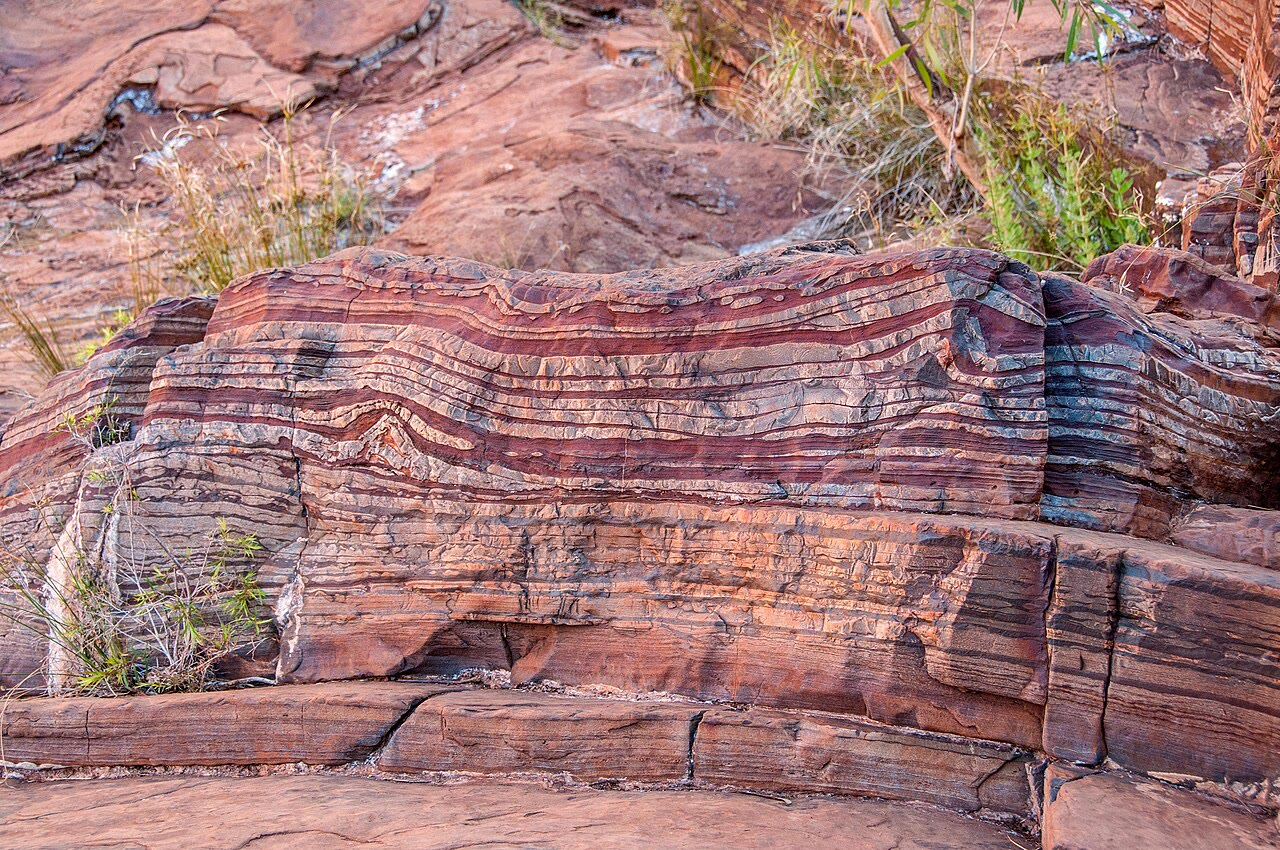
\includegraphics[width=0.72\linewidth]{images/book2/g12-dales-gorge-bif.jpg}

{\small \omterm{def:g12:early-earth:bif}{Formasi besi berpita} di Air Terjun Fortescue, Ngarai Dales, Taman
Nasional Karijini, Australia Barat. Foto Graeme Churchard, CC~BY~2.0
(Wikimedia Commons).}
\end{omfigure}

\begin{recall}
Bumi berumur 4.54 miliar tahun (\cref{ch:g12:age-of-the-earth}), dan zirkon
menunjukkan bahwa kerak sudah ada 4.4 miliar tahun yang lalu
(\cref{ch:g12:continental-crust}). \omterm{def:g10:habitable-planet:equilibrium-temperature}{Suhu kesetimbangan} sebuah planet,
$T_{\mathrm{eq}} = \left(S(1-A)/(4\sigma)\right)^{1/4}$, sekitar \qty{255}{K}
untuk Bumi saat ini (\cref{ch:g10:habitable-planet}). Udara kering saat ini
terdiri dari \qty{78}{\percent} nitrogen dan \qty{21}{\percent} oksigen, dan
karbon dioksida serta metana adalah gas rumah kaca; unsur yang mengikat oksigen
teroksidasi (buku-buku kimia). Tumbuhan, alga, dan sianobakteri membuat
makanannya melalui fotosintesis, yang melepaskan oksigen (buku-buku biologi).
\end{recall}
% ledger: usgs:age-earth (Book 1 row), wilde01:zircon, earth:TSI, earth:albedo, air:N2, air:O2

\section{Bumi muda}

Bumi tumbuh melalui akresi benda-benda yang lebih kecil. Sekitar 60 juta tahun
setelah Tata Surya mulai terbentuk, sebuah benda yang mungkin sebesar Mars
menghantamnya, dan bahan yang terlempar ke angkasa membentuk Bulan. Bumi muda
itu panas dan sebagian masih lebur. Bumi mendingin, dan sekitar 4.4 miliar tahun
yang lalu Bumi sudah mempunyai kerak dan samudra: zirkon yang berumur itu
membawa tanda kimia air cair.
% ledger: nasa:moon-formation, wilde01:zircon

\section{Atmosfer purba}

\begin{definition}[Pelepasan gas; atmosfer purba]\label{def:g12:early-earth:primitive-atmosphere}
Yang disebut \emph{pelepasan gas}\index{pelepasan gas} adalah keluarnya gas-gas
yang terlarut di dalam magma, melalui gunung api dan melalui tanah. Yang disebut
\emph{atmosfer purba}\index{atmosfer purba} adalah atmosfer Bumi sebelum
makhluk hidup mengubahnya: terbentuk terutama melalui pelepasan gas, atmosfer
itu mengandung nitrogen, karbon dioksida, dan uap air, lebih banyak karbon
dioksida daripada sekarang, dan hampir tidak mengandung oksigen bebas.
\end{definition}
% ledger: usgs:volcanic-gases (Book 1 row), holland06:stages (stage 1 anoxic), feulner12:fys (more carbon dioxide)

Gunung api masih menunjukkan bagaimana atmosfer seperti itu terbentuk: ketika
magma naik dan tekanannya turun, gas-gas terlarutnya lolos, dan yang paling
melimpah sejauh ini adalah uap air, lalu karbon dioksida. Nitrogen dan karbon
dioksida, gas-gas yang mendominasi udara purba, masih merupakan gas pembawa
nitrogen dan pembawa karbon yang utama di gunung api saat ini. Uap air itu
mengembun menjadi samudra. Oksigen kurang dari \qty{0.001}{\percent} dari
kadarnya dalam udara saat ini.
% ledger: usgs:volcanic-gases (Book 1 row), pk02:anoxic

Matahari muda bersinar kurang terang daripada sekarang. Ketika Matahari
mengubah hidrogen menjadi helium di intinya, inti itu menyusut dan memanas, dan
daya Matahari perlahan-lahan naik.

\begin{proposition}[Luminositas Matahari muda]\label{prop:g12:early-earth:luminosity}
Bila $t_\odot$ umur Matahari sekarang dan $L_\odot$ luminositasnya sekarang,
luminositasnya ketika Matahari berumur $t$ tahun adalah
\[
  L(t) = \frac{L_\odot}{1 + \frac{2}{5}\left(1 - t/t_\odot\right)} .
\]
\end{proposition}
% ledger: gough81:luminosity, connelly12:cai

Pendekatan atas model-model Matahari yang telah dihitung ini di sini diterima
tanpa bukti. Pada saat lahirnya Matahari, $t = 0$, pendekatan itu memberikan
$L = L_\odot/1.4 \approx 0.71\,L_\odot$: Matahari muda sekitar
\qty{30}{\percent} lebih redup.

\begin{example}[Bumi empat miliar tahun yang lalu]\label{ex:g12:early-earth:young-sun}
Ambillah $t_\odot = 4.567$ miliar tahun. Empat miliar tahun yang lalu Matahari
berumur 0.567 miliar tahun, sehingga $1 - t/t_\odot = 4/4.567 \approx 0.876$ dan
$L \approx L_\odot/1.350 \approx 0.741\,L_\odot$. Sinar Matahari yang sampai di
Bumi adalah $0.741 \times 1361 \approx \qty{1008}{W/m^2}$. Dengan \omterm{def:g10:earth-energy-budget:albedo}{albedo} yang
tetap seperti sekarang, \omterm{def:g10:habitable-planet:equilibrium-temperature}{suhu kesetimbangan} sebanding dengan akar pangkat empat
sinar Matahari: $255 \times 0.741^{1/4} \approx 255 \times 0.928 \approx
\qty{237}{K}$, sekitar \qty{-36}{\celsius}.
\end{example}
% values: L_4Ga 0.7406, S_4Ga 1007.9, Teq_today 255.1, Teq_4Ga 236.7 (early_earth.py)

\begin{omfigure}
\begin{tikzpicture}
\begin{axis}[omrecord, scale only axis, width=0.66\linewidth, height=4.6cm,
  xmin=0, xmax=4.6, ymin=225, ymax=295, x dir=reverse, axis y line*=left,
  xlabel={waktu sebelum sekarang (miliar tahun)}, ylabel={suhu (K)},
  xtick={0,0.5,...,4.5}, x tick label style={/pgf/number format/.cd, fixed, precision=1}]
% computed in figdata/grade-12/early_earth.py; ledger: gough81:luminosity, earth:TSI, earth:albedo, earth:Tsurf
\addplot[omDef, line width=1.2pt] table[x=t_Ga, y=Teq] {figdata/out/grade-12-early_earth-sun.dat};
\addplot[omThm, densely dashed, domain=0:4.6, samples=2] {273.15};
\addplot[black!60, densely dotted, domain=0:4.6, samples=2] {288};
\coordinate (teq) at (axis cs:2.6,239);
\coordinate (frz) at (axis cs:2.3,274);
\coordinate (sfc) at (axis cs:2.3,289);
\end{axis}
\begin{axis}[omrecord, scale only axis, width=0.66\linewidth, height=4.6cm,
  xmin=0, xmax=4.6, ymin=0.65, ymax=1.05, x dir=reverse, axis y line*=right, axis x line=none,
  ylabel={luminositas Matahari ($L_\odot$)}, ymajorgrids=false, xmajorgrids=false,
  y tick label style={/pgf/number format/.cd, fixed, fixed zerofill, precision=2}]
\addplot[omProp, line width=0.9pt, densely dashdotted] table[x=t_Ga, y=L] {figdata/out/grade-12-early_earth-sun.dat};
\coordinate (lum) at (axis cs:1.7,0.86);
\end{axis}
\node[font=\scriptsize, text=omDef, anchor=north] at (teq) {suhu kesetimbangan};
\node[font=\scriptsize, text=omThm, anchor=south] at (frz) {air membeku, \qty{273}{K}};
\node[font=\scriptsize, text=black!70, anchor=south] at (sfc) {permukaan rata-rata kini, \qty{288}{K}};
\node[font=\scriptsize, text=omProp, anchor=north west] at (lum) {luminositas (skala kanan)};
\end{tikzpicture}

{\small Matahari muda yang redup: luminositasnya (skala kanan) dan \omterm{def:g10:habitable-planet:equilibrium-temperature}{suhu
kesetimbangan} Bumi dengan \omterm{def:g10:earth-energy-budget:albedo}{albedo} saat ini (skala kiri), mundur sampai lahirnya
Matahari. Dihitung dari Gough (1981) dengan sinar Matahari dan \omterm{def:g10:earth-energy-budget:albedo}{albedo} saat ini.}
\end{omfigure}

\begin{definition}[Masalah Matahari muda yang redup]\label{def:g12:early-earth:faint-young-sun}
Yang disebut \emph{masalah Matahari muda yang redup}\index{masalah Matahari muda yang redup}
adalah pertentangan antara Matahari yang lebih redup pada miliaran
tahun pertama Bumi, yang di bawahnya Bumi dengan atmosfer seperti sekarang akan
membeku, dan batuan, yang menunjukkan bahwa air cair sudah ada.
\end{definition}
% ledger: feulner12:fys

Masalah itu menjadi dikenal luas pada tahun 1972 melalui Carl Sagan dan George
Mullen, yang mengusulkan efek rumah kaca yang lebih kuat sebagai jawabannya.
Sebagian besar jawaban yang dikaji sejak itu bertumpu pada lebih banyak gas
rumah kaca di dalam \omterm{def:g12:early-earth:primitive-atmosphere}{atmosfer purba}: karbon dioksida yang jauh lebih banyak
daripada sekarang, metana yang dibuat oleh mikroba awal, atau keduanya. Dalam
satu perhitungan klasik, sekitar sepersepuluh bar karbon dioksida, dengan
sedikit metana, menjaga Bumi muda sehangat sekarang; tanpa metana, diperlukan
sekitar tiga kali lebih banyak. Masalah itu belum dianggap terpecahkan.
% ledger: feulner12:fys

\section{Kehidupan dan oksigen}

Rekaman fosil \omterm{def:g12:early-earth:stromatolite}{stromatolit} meliputi hampir \num{3500} juta tahun: \omterm{def:g12:early-earth:stromatolite}{stromatolit}
termasuk tanda-tanda kehidupan yang tertua.

\begin{definition}[Stromatolit]\label{def:g12:early-earth:stromatolite}
Yang disebut \emph{stromatolit}\index{stromatolit} adalah gundukan berlapis yang
dibangun di air dangkal oleh hamparan mikroba, terutama sianobakteri, yang
menjebak dan mengikat butir-butir sedimen dan menumbuhkan karbonat, lapis demi
lapis.
\end{definition}
% ledger: noffke13:stromatolites

\omterm{def:g12:early-earth:stromatolite}{Stromatolit} fosil yang berumur \num{3430} juta tahun dijumpai di Rijang
Strelley Pool di Pilbara, Australia Barat. \omterm{def:g12:early-earth:stromatolite}{Stromatolit} hidup tumbuh saat ini
di air yang sangat asin di Hamelin Pool di Teluk Shark, dua kali lebih asin
daripada air laut biasa, dan di sana \omterm{def:g12:early-earth:stromatolite}{stromatolit} itu menjadi contoh modern yang
paling terkenal.
% ledger: allwood06:spc, noffke13:stromatolites, dbca:hamelin

\begin{omfigure}
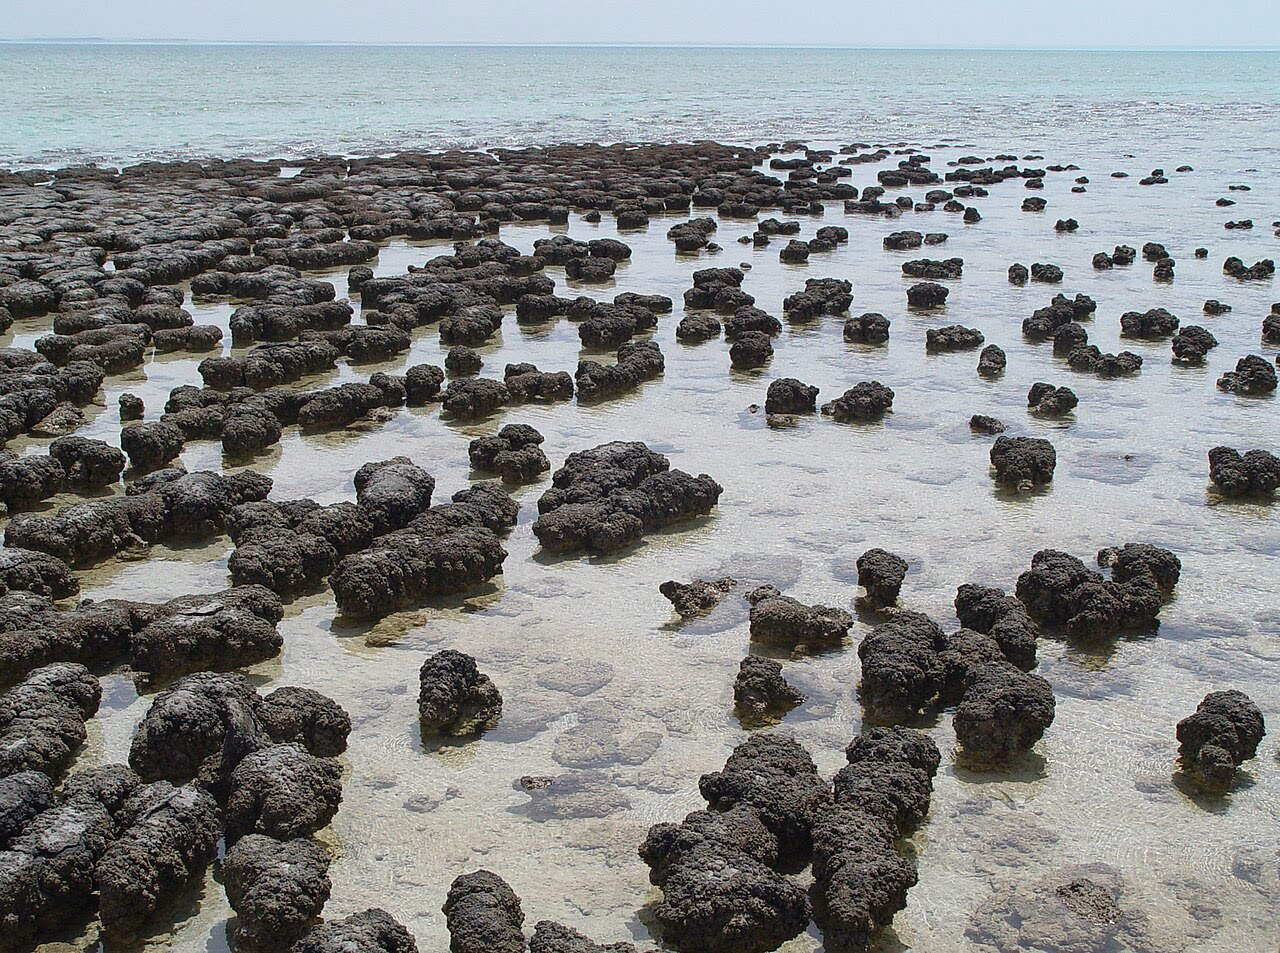
\includegraphics[width=0.6\linewidth]{images/book2/g12-shark-bay-stromatolites.jpg}

{\small \omterm{def:g12:early-earth:stromatolite}{Stromatolit} hidup di Hamelin Pool, Teluk Shark, Australia Barat.
Foto Paul Harrison, CC~BY-SA~3.0 (Wikimedia Commons).}
\end{omfigure}
% ledger: photo:g12-shark-bay

Sianobakteri membawa sesuatu yang baru: fotosintesis yang melepaskan oksigen.
Tetapi untuk waktu yang lama oksigen yang mereka buat tidak tinggal di udara.
Oksigen itu terpakai secepat ia dibuat: oleh besi yang terlarut di laut, oleh
belerang, dan oleh metana.

\section{Naiknya kadar oksigen}

Sebelum ada oksigen, besi dapat berpindah dalam keadaan terlarut di air laut
sebagai ion \ce{Fe^2+}. Oksigen mengubahnya menjadi besi(III), yang tidak larut:
besi itu jatuh ke dasar sebagai sedimen yang berkarat.

\begin{proposition}[Besi mengikat oksigen]\label{prop:g12:early-earth:iron}
Besi(II) terlarut dioksidasi oleh oksigen di dalam air menjadi besi(III)
hidroksida, yang mengendap:
\[
  \ce{4Fe^2+ + O2 + 10H2O -> 4Fe(OH)3 + 8H+} .
\]
Setiap molekul oksigen menghilangkan empat ion besi terlarut; selama masih ada
besi terlarut, oksigen yang dibuat akan terpakai habis.
\end{proposition}
% ledger: earle:bif (ferrous iron oxidised to insoluble ferric iron)

\begin{proof}
Periksalah kesetimbangannya. Besi: 4 di setiap ruas. Oksigen: $2 + 10 = 12$ di
ruas kiri, $4 \times 3 = 12$ di ruas kanan. Hidrogen: $20$ di ruas kiri, $4 \times 3 + 8 =
20$ di ruas kanan. Muatan: $4 \times (+2) = +8$ di ruas kiri, $8 \times (+1) =
+8$ di ruas kanan.
\end{proof}

\begin{definition}[Formasi besi berpita]\label{def:g12:early-earth:bif}
Yang disebut \emph{formasi besi berpita}\index{formasi besi berpita} adalah
batuan sedimen yang tersusun dari lapisan-lapisan tipis yang berselang-seling
antara oksida besi, seperti hematit, dan rijang, yaitu silika berbutir halus
yang miskin besi. Hampir semuanya lebih tua dari 1.8 miliar tahun.
\end{definition}
% ledger: earle:bif, holland06:stages

\omterm{def:g12:early-earth:bif}{Formasi besi berpita} memerlukan dua air sekaligus: \omterm{def:g10:layered-ocean:thermocline}{samudra dalam} tanpa oksigen,
yang membawa besi terlarut, dan laut dangkal yang diterangi Matahari tempat
sianobakteri membuat oksigen dan besi mengendap. Formasi itu umum dijumpai dalam
batuan yang berumur 2.4 sampai 1.8 miliar tahun, dan formasi di Pegunungan
Hamersley bahkan lebih tua lagi. \omterm{def:g12:early-earth:bif}{Formasi besi berpita} adalah bijih besi yang
umum.
% ledger: earle:bif, holland06:stages (Archean BIF, Hamersley), dbca:karijini

\begin{omfigure}
\begin{tikzpicture}[x=1cm, y=1cm, font=\scriptsize]
  % sea and floor
  \fill[omSea] (0,0) rectangle (11,4);
  \fill[omSea!45!white] (0,2.9) rectangle (11,4);
  \draw[omDef!60, line width=0.4pt, densely dashed] (0,2.9) -- (11,2.9);
  \node[anchor=north east, text=omDef] at (10.9,3.95) {air permukaan yang terang};
  \node[anchor=south east, text=omDef, align=right] at (10.9,0.12) {air dalam\\tanpa oksigen,\\kaya \ce{Fe^2+}};
  % floor with layers
  \foreach \i/\c in {0/red!55!black, 1/black!20, 2/red!55!black, 3/black!20, 4/red!55!black, 5/black!20} {
    \fill[\c] (0,-0.12*\i) rectangle (11,-0.12*\i-0.12);
  }
  \draw[black!60] (0,0) -- (11,0);
  \node[anchor=west] at (11.1,-0.12) {oksida besi};
  \node[anchor=west] at (11.1,-0.36) {rijang};
  \draw[black!50, line width=0.3pt] (11.05,-0.06) -- (10.6,-0.06);
  \draw[black!50, line width=0.3pt] (11.05,-0.30) -- (10.6,-0.30);
  % upwelling iron
  \foreach \x in {0.5,1.0,1.5} {
    \draw[-{Stealth}, omDef, line width=0.8pt] (\x,0.4) .. controls (\x+0.4,1.5) and (\x+0.6,2.2) .. (\x+0.9,2.85);
  }
  \node[text=omDef, anchor=west] at (2.3,1.3) {\ce{Fe^2+} naik};
  % cyanobacteria and oxygen
  \foreach \x in {3.8,4.4,5.0,5.6,6.2} {\fill[green!45!black] (\x,3.35) circle (0.07);}
  \node[anchor=south, text=green!35!black] at (5.0,3.47) {sianobakteri membuat \ce{O2}};
  % reaction
  \node[draw=black!40, fill=white, rounded corners=2pt, inner sep=2pt] at (5.4,2.45) {\ce{4Fe^2+ + O2 + 10H2O -> 4Fe(OH)3 + 8H+}};
  % falling rust
  \foreach \x/\y in {4.6/1.9, 5.0/1.5, 5.5/1.8, 5.9/1.2, 4.3/1.1, 5.2/0.7, 6.1/0.6} {\fill[red!60!black] (\x,\y) circle (0.06);}
  \draw[-{Stealth}, red!60!black, line width=0.6pt] (6.6,2.1) -- (6.6,0.25);
  \node[anchor=west, text=red!60!black, align=left] at (6.7,1.75) {besi(III) mengendap\\sebagai lapisan karat};
\end{tikzpicture}

{\small Bagaimana \omterm{def:g12:early-earth:bif}{formasi besi berpita} terbentuk (skematis, tidak berskala):
besi yang terlarut di air dalam, yang tidak mengandung oksigen, naik ke laut
yang diterangi Matahari, tempat oksigen yang dibuat oleh sianobakteri
mengubahnya menjadi besi(III), yang lalu mengendap. Lapisan yang kaya besi
berselang-seling dengan lapisan rijang.}
\end{omfigure}

Lalu oksigen mulai tinggal di udara.

\begin{definition}[Peristiwa Oksidasi Besar]\label{def:g12:early-earth:goe}
Yang disebut \emph{Peristiwa Oksidasi Besar}\index{Peristiwa Oksidasi Besar}
adalah selang waktu, dari sekitar \num{2.46} sampai sekitar \num{2.06} miliar
tahun yang lalu, ketika oksigen bebas untuk pertama kalinya menumpuk di
atmosfer dan laut dangkal Bumi, mencapai mungkin sepersepuluh kadarnya
sekarang.
\end{definition}
% ledger: gumsley17:goe, holland06:stages (0.02-0.04 atm, about a tenth of 0.21)

Buktinya ada di dalam batuan. Sebagian mineral, di antaranya pirit dan
uraninit, dihancurkan oleh oksigen; namun butir-butirnya, yang digulirkan
sungai, dijumpai di dalam sedimen tua, dan butir pirit tidak ada di dalam
sedimen yang diendapkan setelah naiknya kadar oksigen. Isotop belerang dalam
batuan yang lebih tua dari sekitar 2.45 miliar tahun membawa sebuah tanda yang
hanya dapat ditinggalkan oleh udara dengan oksigen kurang dari seperseratus ribu
kadar saat ini; pada 2.09 miliar tahun yang lalu tanda itu telah lenyap. Dan di
daratan muncul \omterm{def:g12:early-earth:red-beds}{lapisan merah}.
% ledger: kasting25:indicators, pk02:anoxic, farquhar00:sulfur

\begin{definition}[Lapisan merah]\label{def:g12:early-earth:red-beds}
Yang disebut \emph{lapisan merah}\index{lapisan merah} adalah batuan sedimen ---
batu pasir, batu lanau, serpih --- yang berwarna merah karena butir-butirnya
diselubungi oksida besi(III), yaitu hematit. Lapisan merah hanya terbentuk di
tempat yang cukup oksigen untuk mengoksidasi besi.
\end{definition}
% ledger: kasting25:indicators (redbeds an oxygen indicator)

\begin{omfigure}
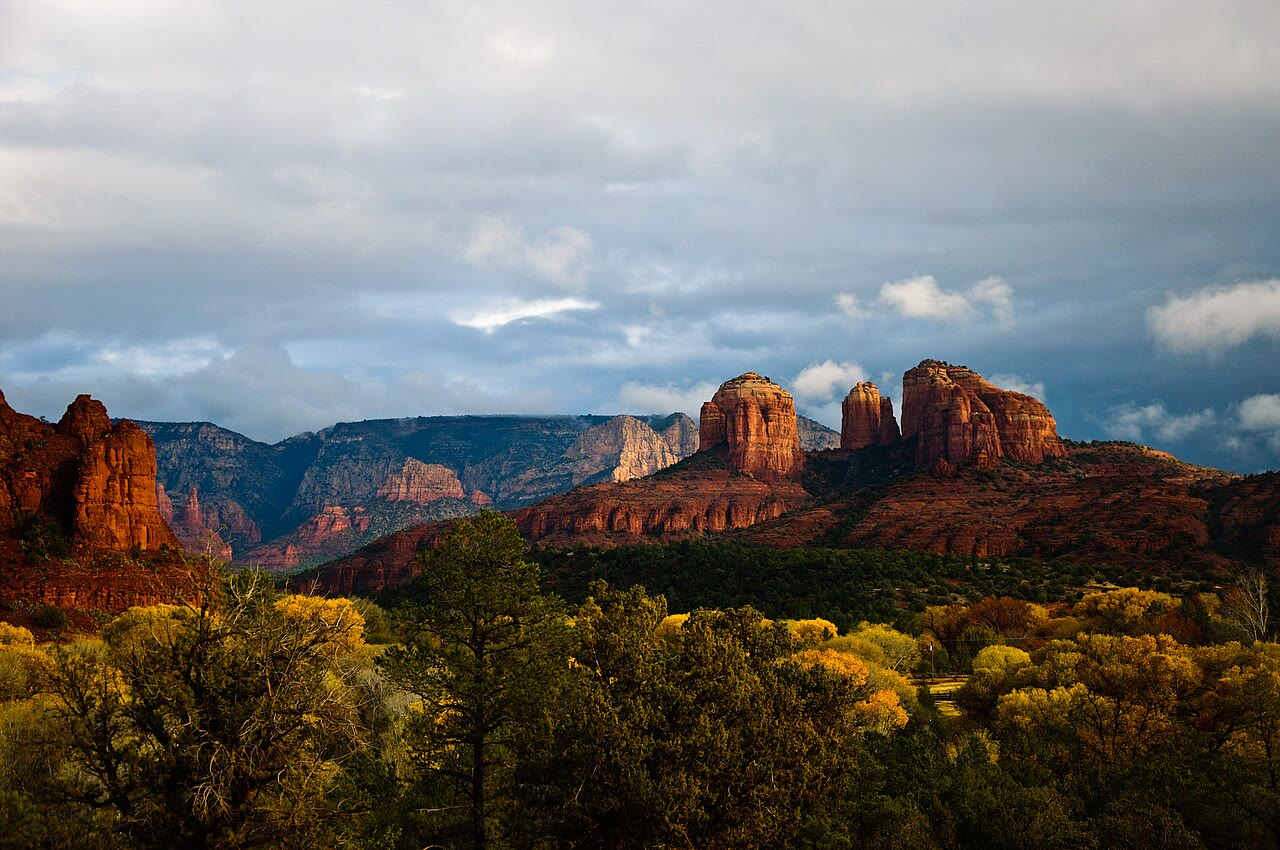
\includegraphics[width=0.66\linewidth]{images/book2/g12-sedona-red-beds.jpg}

{\small \omterm{def:g12:early-earth:red-beds}{Lapisan merah}: Cathedral Rock di dekat Sedona, Arizona, yang tersusun
dari batu pasir merah berumur Perm. Foto Wendy from Pennsylvania, CC~BY-SA~2.0
(Wikimedia Commons).}
\end{omfigure}
% ledger: photo:g12-sedona, azgs:cathedral (Permian Schnebly Hill Sandstone)

Pembentukan \omterm{def:g12:early-earth:bif}{formasi besi berpita} pada dasarnya berhenti setelah 1.8 miliar
tahun yang lalu: pada waktu itu \omterm{def:g10:layered-ocean:thermocline}{samudra dalam} pun sudah cukup mengandung oksigen
sehingga tidak lagi membawa besi. Selama satu miliar tahun berikutnya kadar
oksigen hanya sedikit berubah; setelah 0.85 miliar tahun yang lalu oksigen
kembali menumpuk, menuju \qty{21}{\percent} seperti sekarang.
% ledger: earle:bif, holland06:stages

\begin{method}[Membaca garis waktu geologi]\label{met:g12:early-earth:timeline}
\begin{enumerate}
  \item Tentukan ke arah mana waktu berjalan pada sumbu, dan satuannya (juta
        atau miliar tahun sebelum sekarang).
  \item Temukan kurun-kurun pada pita berwarna, dan bacalah batas-batasnya.
  \item Untuk setiap peristiwa, bacalah tanggalnya, atau selang waktu ketika
        peristiwa itu terjadi, dan katakan rekaman apa yang menanggalinya
        (mineral, fosil, batuan).
  \item Hitung lamanya dengan pengurangan, dan bandingkan dengan \omterm{def:g12:age-of-the-earth:age}{umur Bumi}.
  \item Periksalah urutannya: akibat tidak boleh datang sebelum sebabnya.
\end{enumerate}
\end{method}

\begin{omfigure}
\begin{tikzpicture}
\begin{axis}[omrecord, width=0.82\linewidth, height=6.2cm, ymode=log, xmin=0, xmax=4.6, ymin=1e-7, ymax=5,
  x dir=reverse, xlabel={waktu sebelum sekarang (miliar tahun)}, ylabel={oksigen di udara (kini $=1$)},
  xtick={0,0.5,...,4.5}, x tick label style={/pgf/number format/.cd, fixed, precision=1},
  ytick={1e-6,1e-4,1e-2,1}, ymajorgrids=true, xmajorgrids=false, clip=false]
% computed in figdata/grade-12/early_earth.py (schematic through the sourced bounds); ledger: holland06:stages, pk02:anoxic, gumsley17:goe, ics:base.Hadean, ics:base.Archean, ics:base.Proterozoic, ics:base.Paleozoic
\fill[omThm!12] (axis cs:2.46,1e-7) rectangle (axis cs:2.06,5);
\addplot[black, line width=1.2pt] table[x=t_Ga, y=pal] {figdata/out/grade-12-early_earth-oxygen.dat};
% eon band (ICS colours), below the axis
\fill[icsHadean] (axis cs:4.567,1.5e-7) rectangle (axis cs:4.031,4e-7);
\fill[icsArchean] (axis cs:4.031,1.5e-7) rectangle (axis cs:2.5,4e-7);
\fill[icsProterozoic] (axis cs:2.5,1.5e-7) rectangle (axis cs:0.5388,4e-7);
\fill[icsPhanerozoic] (axis cs:0.5388,1.5e-7) rectangle (axis cs:0,4e-7);
\node[font=\tiny, text=white] at (axis cs:4.30,2.45e-7) {Hadean};
\node[font=\tiny, text=white] at (axis cs:3.27,2.45e-7) {Arkean};
\node[font=\tiny, text=white] at (axis cs:1.52,2.45e-7) {Proterozoikum};
% events
\draw[omDef, line width=0.6pt] (axis cs:4.4,4e-7) -- (axis cs:4.4,3e-3);
\node[font=\scriptsize, text=omDef, anchor=south west] at (axis cs:4.4,3e-3) {zirkon, air};
\draw[omMeth, line width=0.6pt] (axis cs:3.43,4e-7) -- (axis cs:3.43,1.2e-6);
\node[font=\scriptsize, text=omMeth, anchor=south] at (axis cs:3.43,1.2e-6) {stromatolit pertama};
\draw[red!60!black, line width=3pt] (axis cs:2.4,3e-6) -- (axis cs:1.8,3e-6);
\node[font=\scriptsize, text=red!60!black, anchor=north] at (axis cs:2.16,2.4e-6) {formasi besi berpita};
\node[font=\scriptsize, text=omThm, anchor=south, align=center] at (axis cs:2.26,1.2) {Peristiwa Oksidasi\\Besar};
\node[font=\scriptsize, anchor=south] at (axis cs:3.2,1.3e-5) {kurang dari $10^{-5}$ kadar kini};
\node[font=\scriptsize, anchor=south] at (axis cs:1.4,0.12) {sekitar sepersepuluh};
\end{axis}
\end{tikzpicture}

{\small Oksigen di udara sepanjang waktu (skematis, skala logaritmik): kurva itu
menghubungkan batas-batas yang terukur dan menyembunyikan naik turunnya rekaman
yang sebenarnya. Selang yang diarsir adalah \omterm{def:g12:early-earth:goe}{Peristiwa Oksidasi Besar}; batang
merah menandai masa ketika \omterm{def:g12:early-earth:bif}{formasi besi berpita} umum dijumpai, 2.4 sampai 1.8
miliar tahun yang lalu. Kurun-kurun dari Bagan Kronostratigrafi
Internasional.}
\end{omfigure}

\section{Latihan}

\begin{exercise}[$\star$]\label{exo:g12:early-earth:1}
Sebutkan istilahnya: (a) keluarnya gas-gas yang terlarut di dalam magma;
(b) gundukan berlapis yang dibangun oleh hamparan mikroba; (c) batuan yang
tersusun dari lapisan oksida besi dan rijang yang berselang-seling; (d) batuan
sedimen yang diwarnai hematit; (e) selang waktu ketika oksigen untuk pertama
kalinya menumpuk di udara.
\end{exercise}

\begin{exercise}[$\star$]\label{exo:g12:early-earth:2}
Urutkan, mulai dari yang tertua: berakhirnya sebagian besar \omterm{def:g12:early-earth:bif}{formasi besi
berpita}; \omterm{def:g12:early-earth:stromatolite}{stromatolit} pertama di Pilbara; zirkon yang menunjukkan air cair;
\omterm{def:g12:early-earth:bif}{formasi besi berpita} Hamersley; berakhirnya \omterm{def:g12:early-earth:goe}{Peristiwa Oksidasi Besar}.
\end{exercise}

\begin{exercise}[$\star$]\label{exo:g12:early-earth:3}
Dengan hukum luminositas, hitung luminositas Matahari pada saat lahirnya,
sebagai bagian dari luminositasnya sekarang. Berapa persen lebih redup
Matahari waktu itu?
\end{exercise}

\begin{exercise}[$\star$]\label{exo:g12:early-earth:4}
Butir-butir pirit yang digulirkan sungai dijumpai di dalam sedimen tua, tetapi
tidak di dalam sedimen yang diendapkan setelah naiknya kadar oksigen. Apa yang
dikatakan hal ini kepadamu tentang udara pada masa sedimen tua itu? Mengapa?
\end{exercise}

\begin{exercise}[$\star$]\label{exo:g12:early-earth:5}
Sebutkan dua gas paling melimpah yang dilepaskan gunung api, dan katakan apa
yang terjadi pada masing-masing di Bumi muda.
\end{exercise}

\begin{exercise}[$\star\star$]\label{exo:g12:early-earth:6}
Hitung luminositas Matahari dan \omterm{def:g10:habitable-planet:equilibrium-temperature}{suhu kesetimbangan} Bumi (saat ini
\qty{255}{K}, \omterm{def:g10:earth-energy-budget:albedo}{albedo} tidak berubah) 3 miliar tahun yang lalu dan 2.45 miliar
tahun yang lalu, dengan mengambil $t_\odot = 4.567$ miliar tahun.
\end{exercise}

\begin{exercise}[$\star\star$]\label{exo:g12:early-earth:7}
Berapa banyak oksigen yang diperlukan untuk mengendapkan \qty{1}{kg} besi
terlarut sebagai besi(III) hidroksida? (Massa molar: besi \qty{55.85}{g/mol},
oksigen \qty{16.00}{g/mol}.)
\end{exercise}

\begin{exercise}[$\star\star$]\label{exo:g12:early-earth:8}
Dengan garis waktu itu, (1) berapa lama \omterm{def:g12:early-earth:goe}{Peristiwa Oksidasi Besar} berlangsung?
(2) Selama berapa bagian sejarah Bumi udara hampir tidak mengandung oksigen?
(3) Berapa lama setelah \omterm{def:g12:early-earth:stromatolite}{stromatolit} pertama oksigen mulai menumpuk?
\end{exercise}

\begin{exercise}[$\star\star$]\label{exo:g12:early-earth:9}
\omterm{def:g12:early-earth:bif}{Formasi besi berpita} dan \omterm{def:g12:early-earth:red-beds}{lapisan merah} sama-sama mengandung oksida besi(III).
Apa yang dikatakan masing-masing kepadamu tentang oksigen, dan di mana: di laut
dalam, di laut dangkal, di udara?
\end{exercise}

\begin{exercise}[$\star\star$]\label{exo:g12:early-earth:10}
Di mana \omterm{def:g12:early-earth:stromatolite}{stromatolit} hidup dapat dilihat saat ini? Apa yang istimewa dari air di
sana, dan bagaimana \omterm{def:g12:early-earth:stromatolite}{stromatolit} tumbuh lapis demi lapis?
\end{exercise}

\begin{exercise}[$\star\star$]\label{exo:g12:early-earth:11}
Oksigen merupakan \qty{21}{\percent} udara saat ini. Berapa persen kadarnya
ketika oksigen itu (1) seperseratus ribu kadar saat ini; (2) sepersepuluh kadar
saat ini?
\end{exercise}

\begin{exercise}[$\star\star\star$]\label{exo:g12:early-earth:12}
Empat miliar tahun yang lalu, \omterm{def:g10:earth-energy-budget:albedo}{albedo} berapa yang akan memberikan \omterm{def:g10:habitable-planet:equilibrium-temperature}{suhu
kesetimbangan} Bumi seperti sekarang, \qty{255}{K}, di bawah Matahari muda
($L = 0.741\,L_\odot$, \omterm{def:g10:earth-energy-budget:albedo}{albedo} saat ini 0.294)? Mungkinkah sebuah planet yang
mempunyai samudra, awan, dan sedikit es segelap itu? Apa jalan keluar yang
lain?
\end{exercise}

\begin{exercise}[$\star\star\star$]\label{exo:g12:early-earth:13}
Saat ini efek rumah kaca menghangatkan permukaan Bumi dari 255 menjadi
\qty{288}{K}. Empat miliar tahun yang lalu \omterm{def:g10:habitable-planet:equilibrium-temperature}{suhu kesetimbangannya} sekitar
\qty{237}{K}. (1) Berapa kelvin pemanasan rumah kaca yang diperlukan waktu itu
untuk mencapai \qty{273}{K}? Untuk mencapai \qty{288}{K}? (2) Bandingkan
dengan pemanasan saat ini. (3) Satu perhitungan klasik memerlukan sekitar
\qty{0.1}{bar} karbon dioksida, dengan sedikit metana; bandingkan dengan
tekanan seluruh atmosfer saat ini, sekitar \qty{1}{bar}.
\end{exercise}

\begin{exercise}[$\star\star\star$]\label{exo:g12:early-earth:14}
Sebuah tanda khusus isotop belerang hanya dapat dibuat, dan tersimpan di dalam
sedimen, bila udara mengandung oksigen kurang dari $10^{-5}$ kadar saat ini.
Tanda itu dijumpai di dalam batuan yang lebih tua dari 2450 juta tahun, dan
tidak di dalam batuan yang lebih muda dari 2090 juta tahun. (1) Apa
kesimpulanmu tentang oksigen sebelum 2450 juta tahun yang lalu? Setelah 2090
juta tahun? (2) Apakah hal ini sesuai dengan tanggal-tanggal \omterm{def:g12:early-earth:goe}{Peristiwa Oksidasi
Besar}?
\end{exercise}

\begin{exercise}[$\star\star\star$]\label{exo:g12:early-earth:15}
Tumbukan yang membentuk Bulan terjadi sekitar 60 juta tahun setelah Tata Surya
mulai terbentuk, yang menurut zat padat pertamanya terjadi 4567 juta tahun yang
lalu. (1) Kira-kira kapan tumbukan itu terjadi? (2) Zirkon tertua berumur
\num{4404} juta tahun. Paling lama berapa waktu setelah tumbukan itu Bumi sudah
mempunyai kerak padat dan air cair?
\end{exercise}
% ledger: nasa:moon-formation, connelly12:cai, wilde01:4404

\begin{problem}[{Soal akhir pekan --- Matahari muda yang redup}]
\label{pb:g12:early-earth:1}
% ledger: gough81:luminosity, connelly12:cai, earth:TSI, earth:albedo, earth:Tsurf, feulner12:fys, allwood06:spc, dbca:karijini, wilde01:zircon
% values (early_earth.py): L_4Ga 0.7406, S_4Ga 1007.9, Teq_today 255.1, Teq_4Ga 236.7, albedo_needed 0.047
Matahari berumur \num{4.567} miliar tahun. Luminositasnya ketika berumur $t$
tahun adalah $L(t) = L_\odot/\bigl(1 + \tfrac25 (1 - t/t_\odot)\bigr)$. Saat
ini Bumi menerima \qty{1361}{W/m^2} sinar Matahari, memantulkan bagian 0.294
darinya, dan mempunyai \omterm{def:g10:habitable-planet:equilibrium-temperature}{suhu kesetimbangan} \qty{255}{K}; suhu permukaan
rata-ratanya \qty{288}{K}.

\medskip
\noindent\textbf{Bagian I --- Matahari empat miliar tahun yang lalu.}
\begin{enumerate}
  \item Berapa umur Matahari empat miliar tahun yang lalu?
  \item Hitung $1 - t/t_\odot$ pada waktu itu.
  \item Hitung luminositasnya sebagai bagian dari luminositas sekarang.
  \item Berapa sinar Matahari yang diterima Bumi, dalam \unit{W/m^2}?
  \item Berapa persen Matahari lebih redup daripada sekarang?
\end{enumerate}

\medskip
\noindent\textbf{Bagian II --- Suhu kesetimbangan.}
\begin{enumerate}[resume]
  \item Tuliskan \omterm{def:g10:habitable-planet:equilibrium-temperature}{suhu kesetimbangan} sebagai fungsi sinar Matahari $S$.
  \item Tunjukkan bahwa, dengan \omterm{def:g10:earth-energy-budget:albedo}{albedo} yang tidak berubah, suhu itu berubah
        sebanding dengan $S^{1/4}$.
  \item Hitung $0.741^{1/4}$.
  \item Hitung \omterm{def:g10:habitable-planet:equilibrium-temperature}{suhu kesetimbangan} empat miliar tahun yang lalu.
  \item Ubahlah ke derajat Celsius.
\end{enumerate}

\medskip
\noindent\textbf{Bagian III --- Bukti adanya air cair.}
\begin{enumerate}[resume]
  \item Apa yang ditunjukkan oleh zirkon yang berumur 4.4 miliar tahun?
  \item Di air seperti apa \omterm{def:g12:early-earth:stromatolite}{stromatolit} Pilbara, yang berumur \num{3430} juta
        tahun, tumbuh?
  \item Batuan apa di Pegunungan Hamersley, yang diendapkan di laut lebih dari
        2.5 miliar tahun yang lalu, yang memerlukan air cair?
  \item Tanpa efek rumah kaca, apakah samudra akan membeku empat miliar tahun
        yang lalu? Mengapa?
  \item Nyatakan pertentangan yang diungkapkan hal ini, dan sebutkan namanya.
\end{enumerate}

\medskip
\noindent\textbf{Bagian IV --- Pemanasan rumah kaca yang diperlukan.}
\begin{enumerate}[resume]
  \item Berapa kelvin yang ditambahkan oleh efek rumah kaca saat ini?
  \item Berapa kelvin yang diperlukan empat miliar tahun yang lalu untuk
        menjaga permukaan rata-rata di atas \qty{273}{K}?
  \item \omterm{def:g10:earth-energy-budget:albedo}{Albedo} berapa yang akan memberikan \qty{255}{K} tanpa efek rumah kaca
        tambahan? Masuk akalkah itu?
  \item Gas apa yang diduga memasok sebagian besar pemanasan tambahan itu, dan
        gas lain apa yang mungkin ikut membantu?
  \item Simpulkan: berapa \omterm{def:g10:habitable-planet:equilibrium-temperature}{suhu kesetimbangan} Bumi empat miliar tahun yang lalu?
\end{enumerate}
\end{problem}
